\chapter{Ergebnisse}
    Innerhalb diese Kapitels geht es zunöchst um die Vorbereitung der Proben.
    Weiter geht es es um den Umgang mit dem dreidimensionalen Datensatz sowie dessen Bearbeitung.
    Die verschiedenen extrahierten Darstellungen werden dann aufgenommen und analysiert.
    In dieser Arbeit untersuchten Proben wurden alle in dem Versuchsaufbau aus \autoref{sec:Versuchsaufbau} vorbereitet und vermessen.

    \section{Vorbereitung und Präperation}
    \label{sec:Praep}
        Zum Präperieren der Proben werden zunächst die verschiedenen Substrate durch mehrfaches ioneninduziertes Zerstäuben und aufheizen gereinigt.
        Für die Goldprobe wurde eine Spannung von \SI{2}{\kilo\volt} und ein Strom von \SI{10}{\milli\ampere}, mit anschließendenem Aufheizen auf etwa \SI{500}{\degree\celsius}.
        Hingegen wurde bei der Eisenprobe nur ein Spannung von \SI{1}{\kilo\volt} gewählt, da es sich um einen dünnen auf Magnesiumoxid gewachsenen Film handelt.
        Allerdings wurde die Probe dann auf etwa \SI{600}{\degree\celsius} aufgeheizt.
        Anschließend wird die Oberflächenstruktur mittels LEED überprüft, dabei ergeben sich die Bilder in \autoref{fig:LEED_samples}.

        Nun wurde auf die Goldprobe ein Nickeloxid-Film aufgebracht, dies geschieht durch das Aufdampfen von Nickel mit einer Rate von \SI{0.3}{\angstrom\per\minute} in einer Sauerstoffatmosphäre von \SI{2e-6}{\milli\bar}.S
        Für den Eisenoxidfilm wird Eisen mit einer Rate von \SI{0.6}{\ML\per\minute} und einem Sauerstoffdruck von \SI{}{\milli\bar} aufgedampft.
        Dabei wird die Probe auf eine Temperatur von \SI{230}{\degree\celsius} gehalten und anschließend bei \SI{650}{\degree\celsius} ausgeheizt.
        Beide Filme werden erneut mittels LEED überprüft, das Eisenoxid zusätzlich mittels Augerelektronenspektroskopie überprüft.
        Anschließend werden die beiden nun antiferromagnnetischen Substrate vermessen und anschließend wird eine Monolage Pentacene aufgedampft.
        Nach dem Aufdampfen wurde versucht ein LEED Bild aufzunehmen, es waren allerdings nur leichte Substratspots sichtbar.
        So lässt sich schlussfolgern, dass sich die Moleküle auf der Oberfläche nicht anordnen.
        

    \section{Datenformat und Bearbeitung}
        Für die Auswertung der dreidimensionalen Datenwird die Software IGOR Pro \cite{IGOR} genutzt.
        Alle Messungen der winkelaufgelösten Bandstruktur wurden als dreidimensionale Datensätze aufgenommen.
        Da die Bilder auf Grund nicht perfekt eingestellter Linsen nicht kreisrund sind, werden die Elipsen angepasst.
        Hierfür wird die kleiner der beiden Achsen entlang der Achse gestreckt.
        Ferner muss der Polarisationsfaktor unter Beachtung der Substratgeometrie kompensiert werden.
        Hierfür werden die Bilder jeweils um \SI{\pm120}{\degree} gedreht und auf das ursprüngliche Bild aufaddiert.
        Um die gemessene kinetische Energie in die relevante Bindungsenergie umzurechnen wird bei den integrierten Spektren aus \autoref{sec:EDC} eine Faltung aus \textbf{...} an die Fermikante durchgeführt.
        Zusätzlich müssen die gemessenen Bilder von ihren Pixelwerten noch in die entsprechenden Impulswerte umgerechnet werden.
        Dies geschieht mit Hilfe der Sekundärelektronen aus dem Spektrum der Austrittsarbeit (niedrige kinetische Energie).
        Ihre kinetische Energie kann durch 
        \begin{equation}
            E_\text{Kin} = \frac{\hbar^2 {k_{||}}^2}{2 m}
            \label{eqn:WKF}
        \end{equation}
        beschrieben werden, wobei $m$ die Elektronenmasse und $k_{||}$ ihr Impuls parallel zur Oberfläche ist.
        Die langsamsten Elektronen treten mit einer kinetischen Energie von \SI{0}{\electronvolt} aus der Probe aus und bilden damit den unteren Punkt der Parabel in \autoref{fig:WKF}.
        Durch ihren parabolischen Verlauf kann nun bei einer höher liegenden Energie ein Linienprofil genommen werden.
        Da sich die Elektronen wie in \autoref{eqn:WKF} verhalten können damit die Pixel in entsprechende Impulswerte umgerechnet werden.


    \section{Integrierte Spektren}
    \label{sec:EDC}
        \begin{wrapfigure}{r}{5cm}
            \centering
            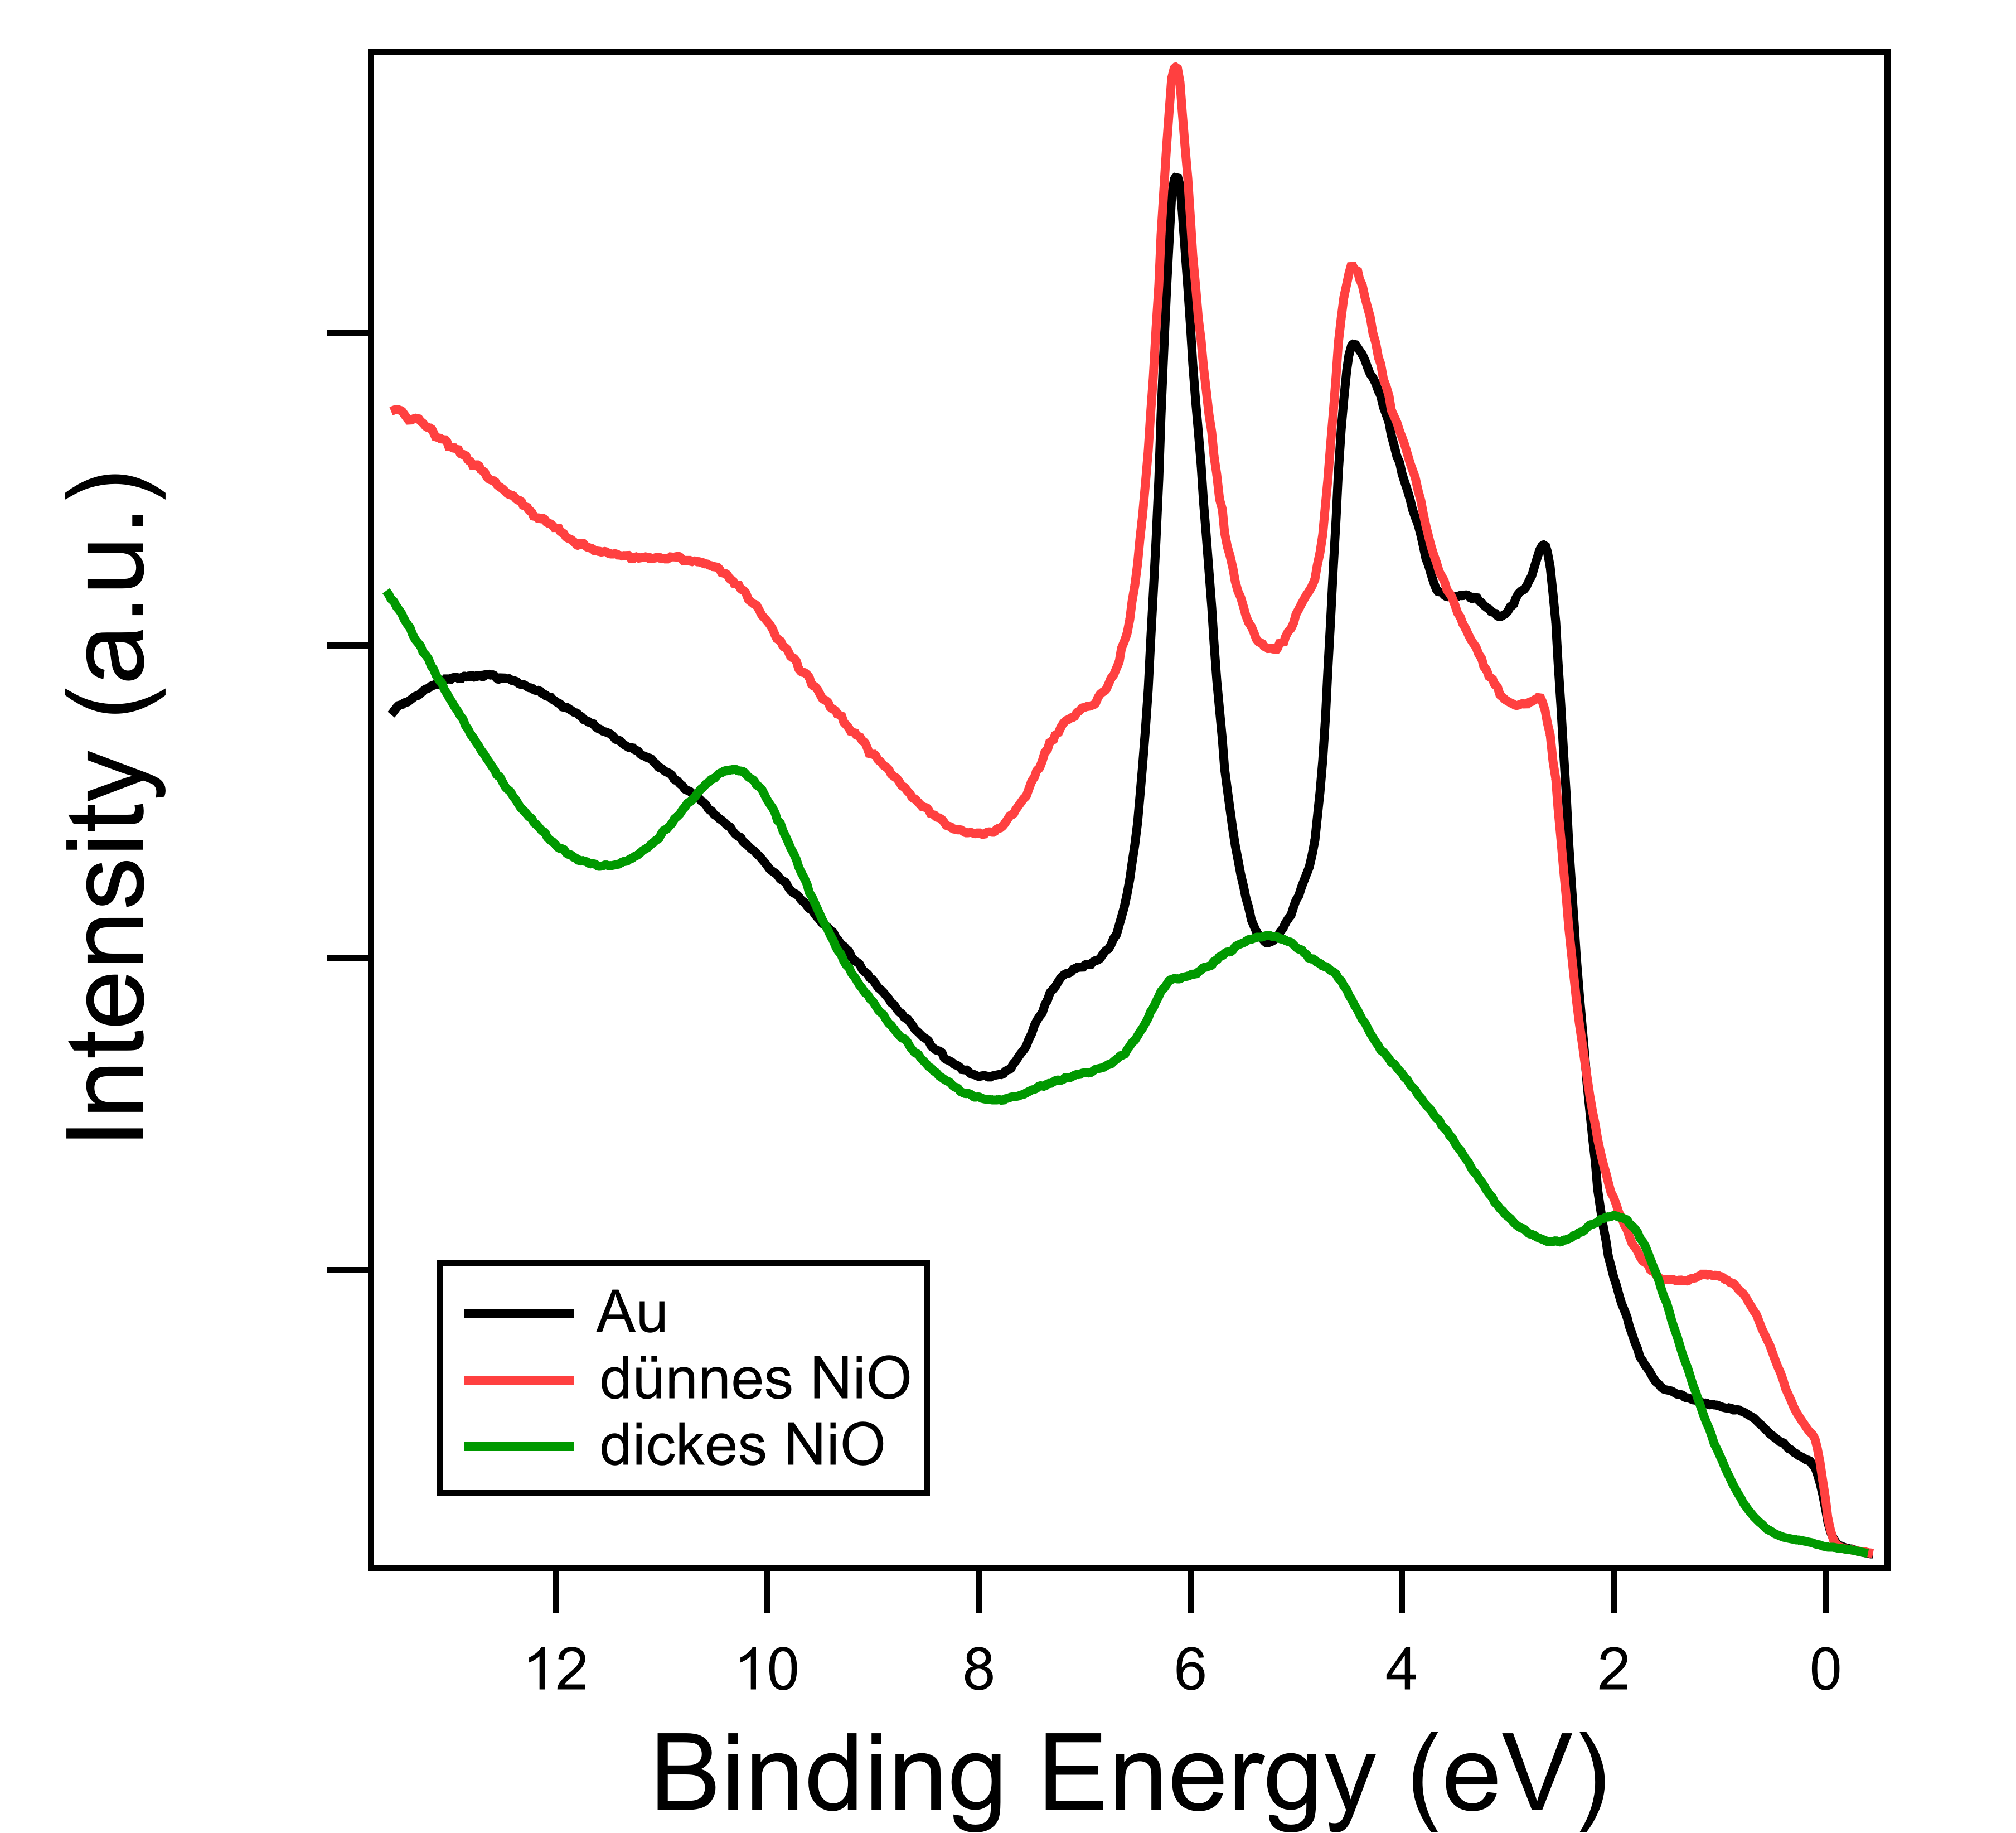
\includegraphics[width=4.5cm]{./content/NiO_Filmdicke}
            \caption{Die integrierten Spektren für zwei verschiedene Schichtdicken von \ce{NiO}. Als Referenz dient das integrierte Spektrum von Gold.}
            \label{fig:NiO_Filmdicke}
        \end{wrapfigure}
        Die Elektronendichtekurven für die reinen Substrate sind gemeinsam mit den der zusätzlich aufgebrachten Molekülen in den Abbildungen~\ref{fig:NiO+5A} und~\ref{fig:FeO+5A} dargestellt.
        Es lassen sich bei den in den Spektren erkennbare zusätzliche Merkmale erkennen die somit den Molekülen zugeordnet werden können.
        An diesen Punkten werden einzelne Bilder mit einer erhöhten Statistik aufgenommen.
        %   \begin{figure}
        %     \centering
        %     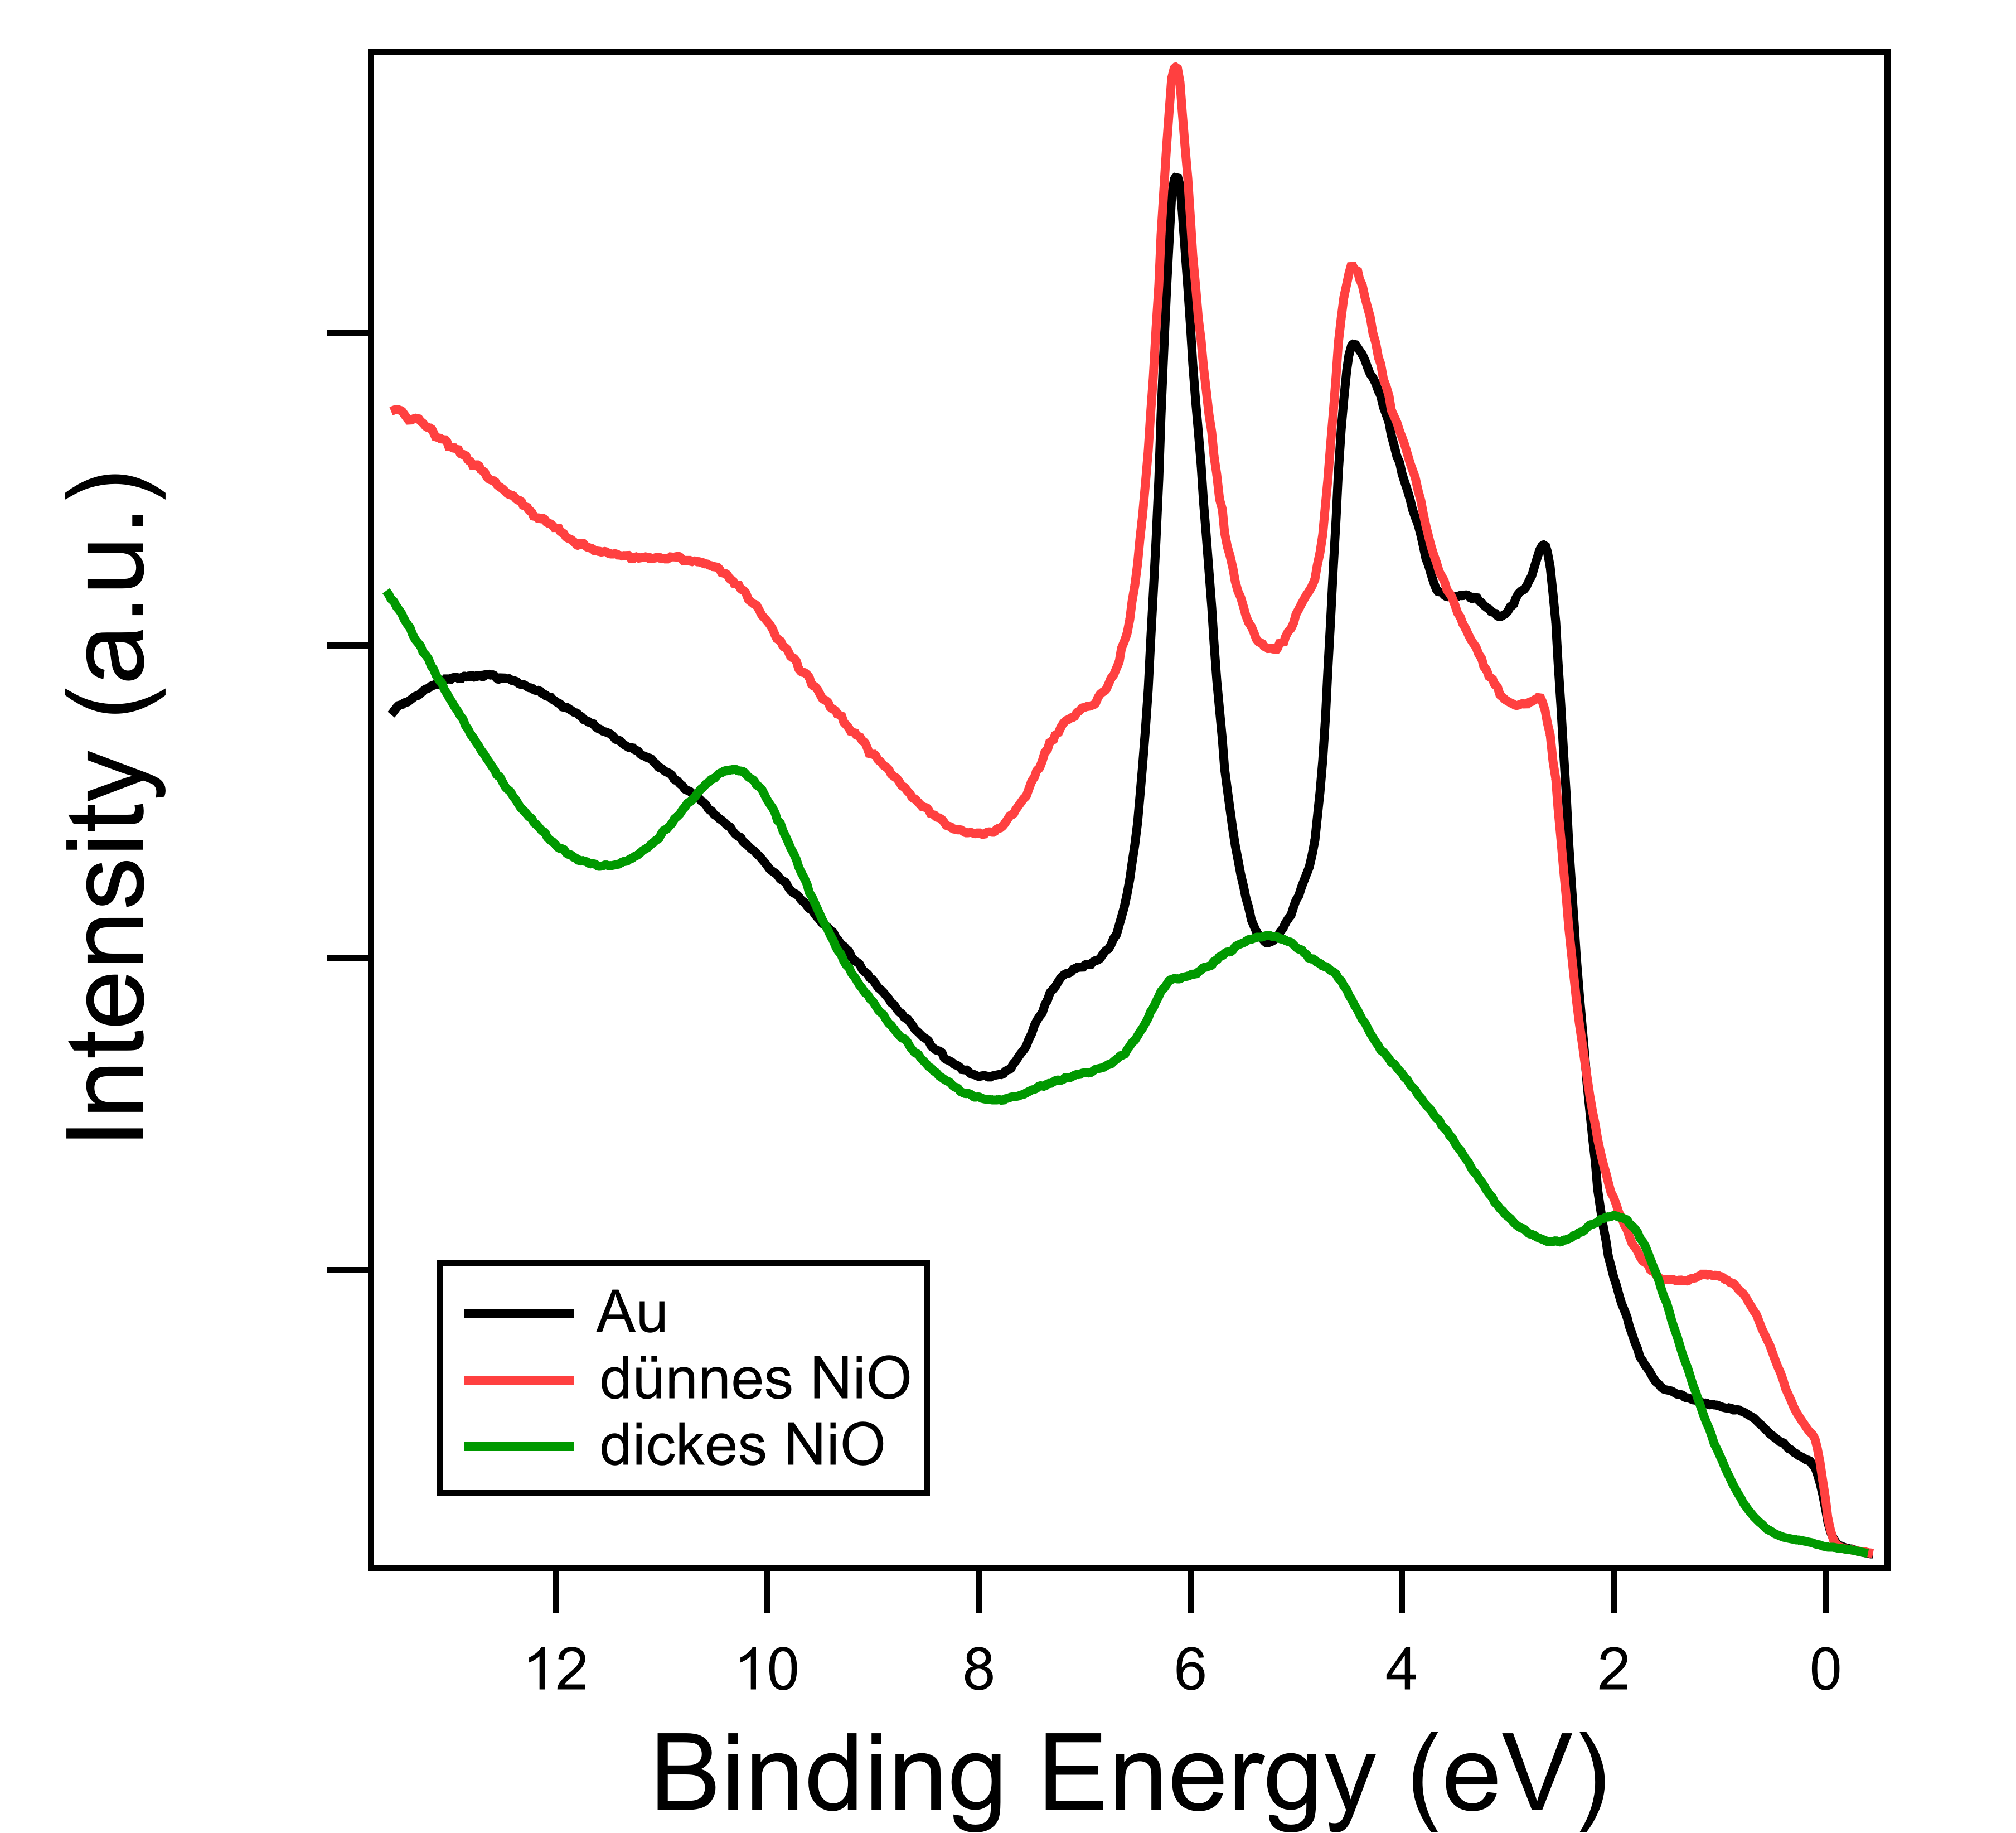
\includegraphics[width=0.7\textwidth]{./content/NiO_Filmdicke.png}
        %     \caption{Das Valenzbandspektrum von Nickeloxid im vergleich zu Messungen aus der Lieteratur.}
        %     \label{fig:NiO_Filmdicke}
        % \end{figure}
        Wird die gesamte Länge des Spektrums betrachtet, also der Energieunterschied zwischen Fermikante und Ende des Sekundärelektronen, so lässt sich die Austrittsarbeit der Probe bestimmen.
        So lässt sich erkennen, dass sich die Austrittsarbeit vom Gold zu dickeren Filmen Nickeloxid zu kleineren Werten verschiebt.
        Für Gold lässt sich die Austrittsarbeit auf \SI{5.46}{\electronvolt} ermitteln, was \textbf{Quelle Hüfner?, Zahl}.
        Vom dünnen Nickeloxidfilm zum dickeren Nickeloxidfilm wechselt sie von \SI{4.25}{\electronvolt} zu \SI{3.90}{\electronvolt}.
        Die Austrittsarbeit des dicken Nickeloxidfilms passt \textbf{Quelle und Wert}.
        Für das Eisenoxid ergibt sich eine Austrittsarbeit von \textbf{Wert sowie Literatur}.


        \begin{itemize}
            \item Sieht Features später Zuordnung
            \item Ändert sich was
        \end{itemize}

    \section{Bandstruktur}
        \begin{itemize}
            \item Bandstruktur von Gold
            \item Bandstruktur NiO? Spin?
            \item Bandstruktur mit Molekülen - Oberflächenzustände? Extra Features
        \end{itemize}

    \section{Maps}
        In den Bildern von Pentacene auf Nickel- und Eisenoxid lassen sich leider keine Molekülorbitale zuordnen.
        Die Ursache ist, dass wie bereits im \autoref{sec:Praep} anhand der LEED Bilder festgestellt wurde, die Moleküle sich nicht regelmäßig auf der Oberfläche anordnen.
        Ferner überlappen dann die einzelnen Merkmale im Impulsraum, sodass ein ausgewaschenes Bild entsteht.

        Wenn hingegen die Moleküle auf dem reinen Goldkristall aufgebracht werden er gibt sich eine periodische Struktur.
        Dies lässt sich anhand von LEED Bildern erkennen, ebenso in der Möglichkeit die Bilder im Impulsraum den theoretisch ermittelten Molekülorbitalen zuzuordnen, wie es in der \autoref{fig:MOT} geschehen ist.
        Hierzu wurden auf die berechneten Bilder die selben symmetrisierungs Schritte angewendet wie auf die gemessenen.

        Der größte Unterschied zwischen dem Gold und den Oxiden ist deren isolierenden Eigenschaften, es lässt sich also vermuten, dass für die Ornung Leitfähigkeit voraus gesetzt wird.


        \begin{itemize}
            \item Maps selbst die sich zuordnen lassen
            \item Aus den LP bestimmte zuordnung möglich?
        \end{itemize}

        \subsection{5A on Au}
        \textbf{6 Bilder in einem Bild}
            \begin{figure}
                \label{fig:MOT}
                \centering
                \begin{subfigure}{0.48\textwidth}
                    \centering
                    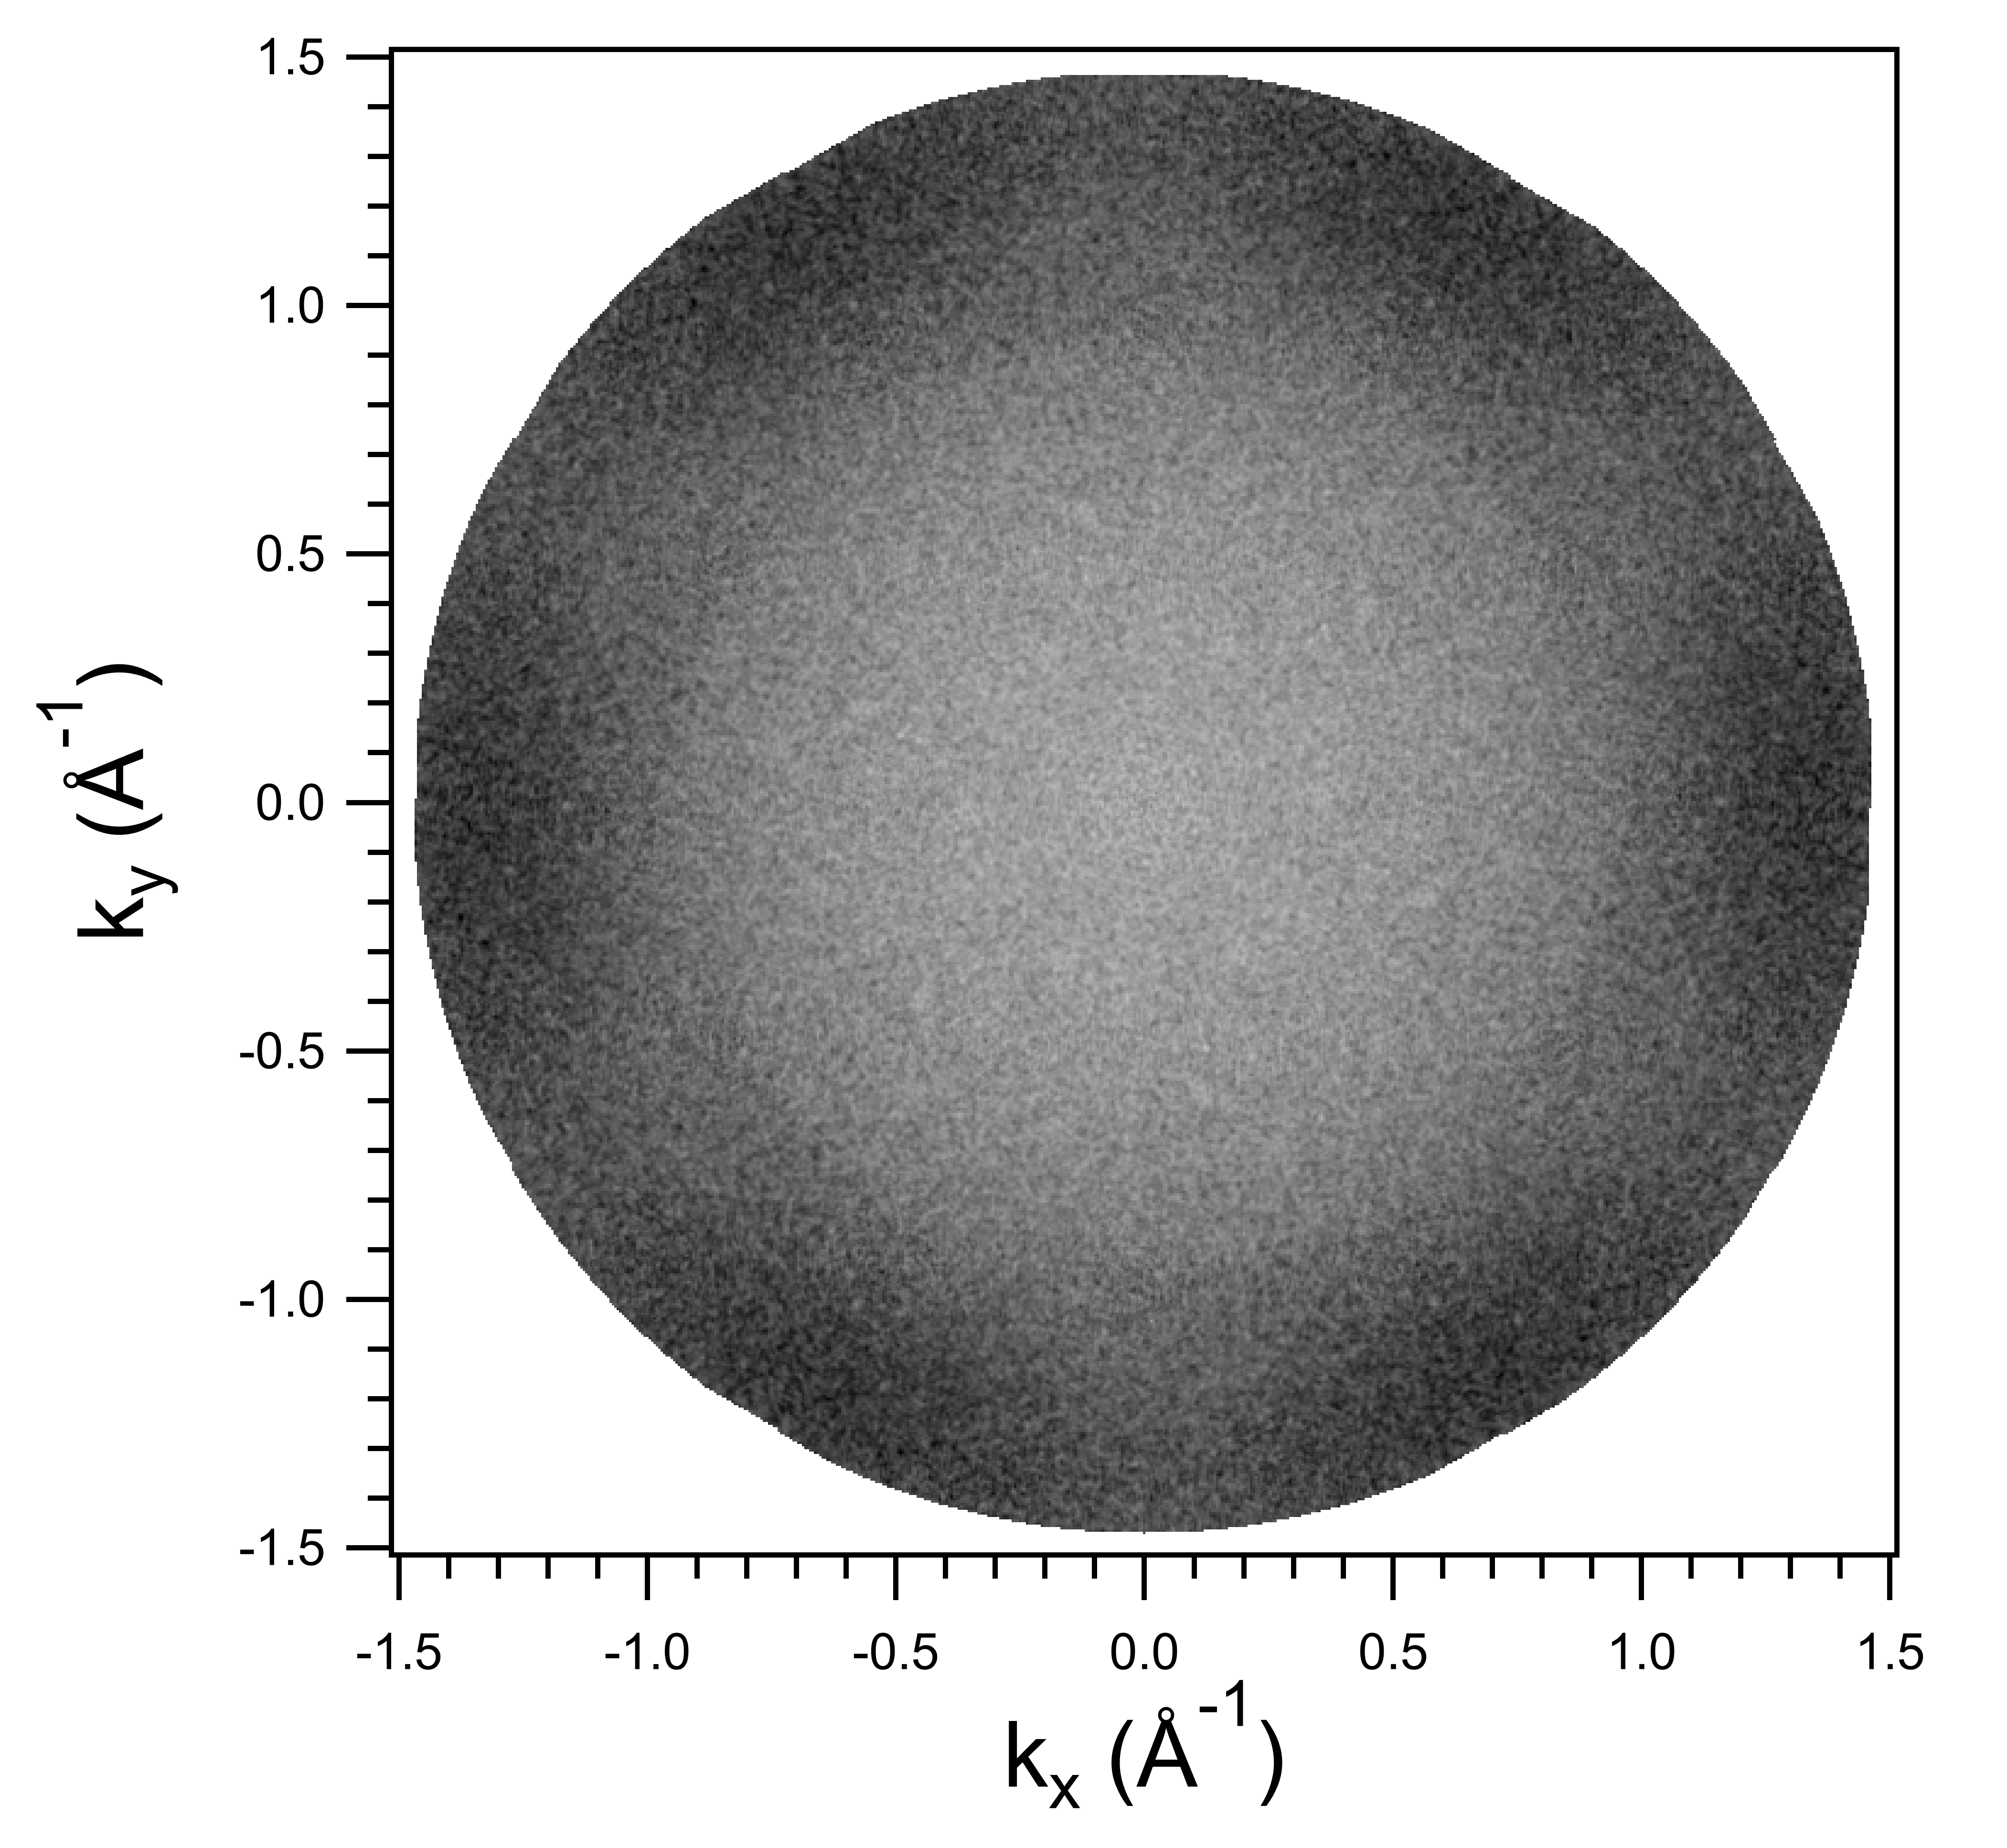
\includegraphics[height=5cm]{./content/Au+5A/IMAGE_2021_06_17_005_BE0_8}
                    \subcaption{Gemmesen, symmetrisiertes Bild bei einer Bindungsenergie von \SI{0.8}{\electronvolt}.}
                \end{subfigure}
                \begin{subfigure}{0.48\textwidth}
                    \centering
                    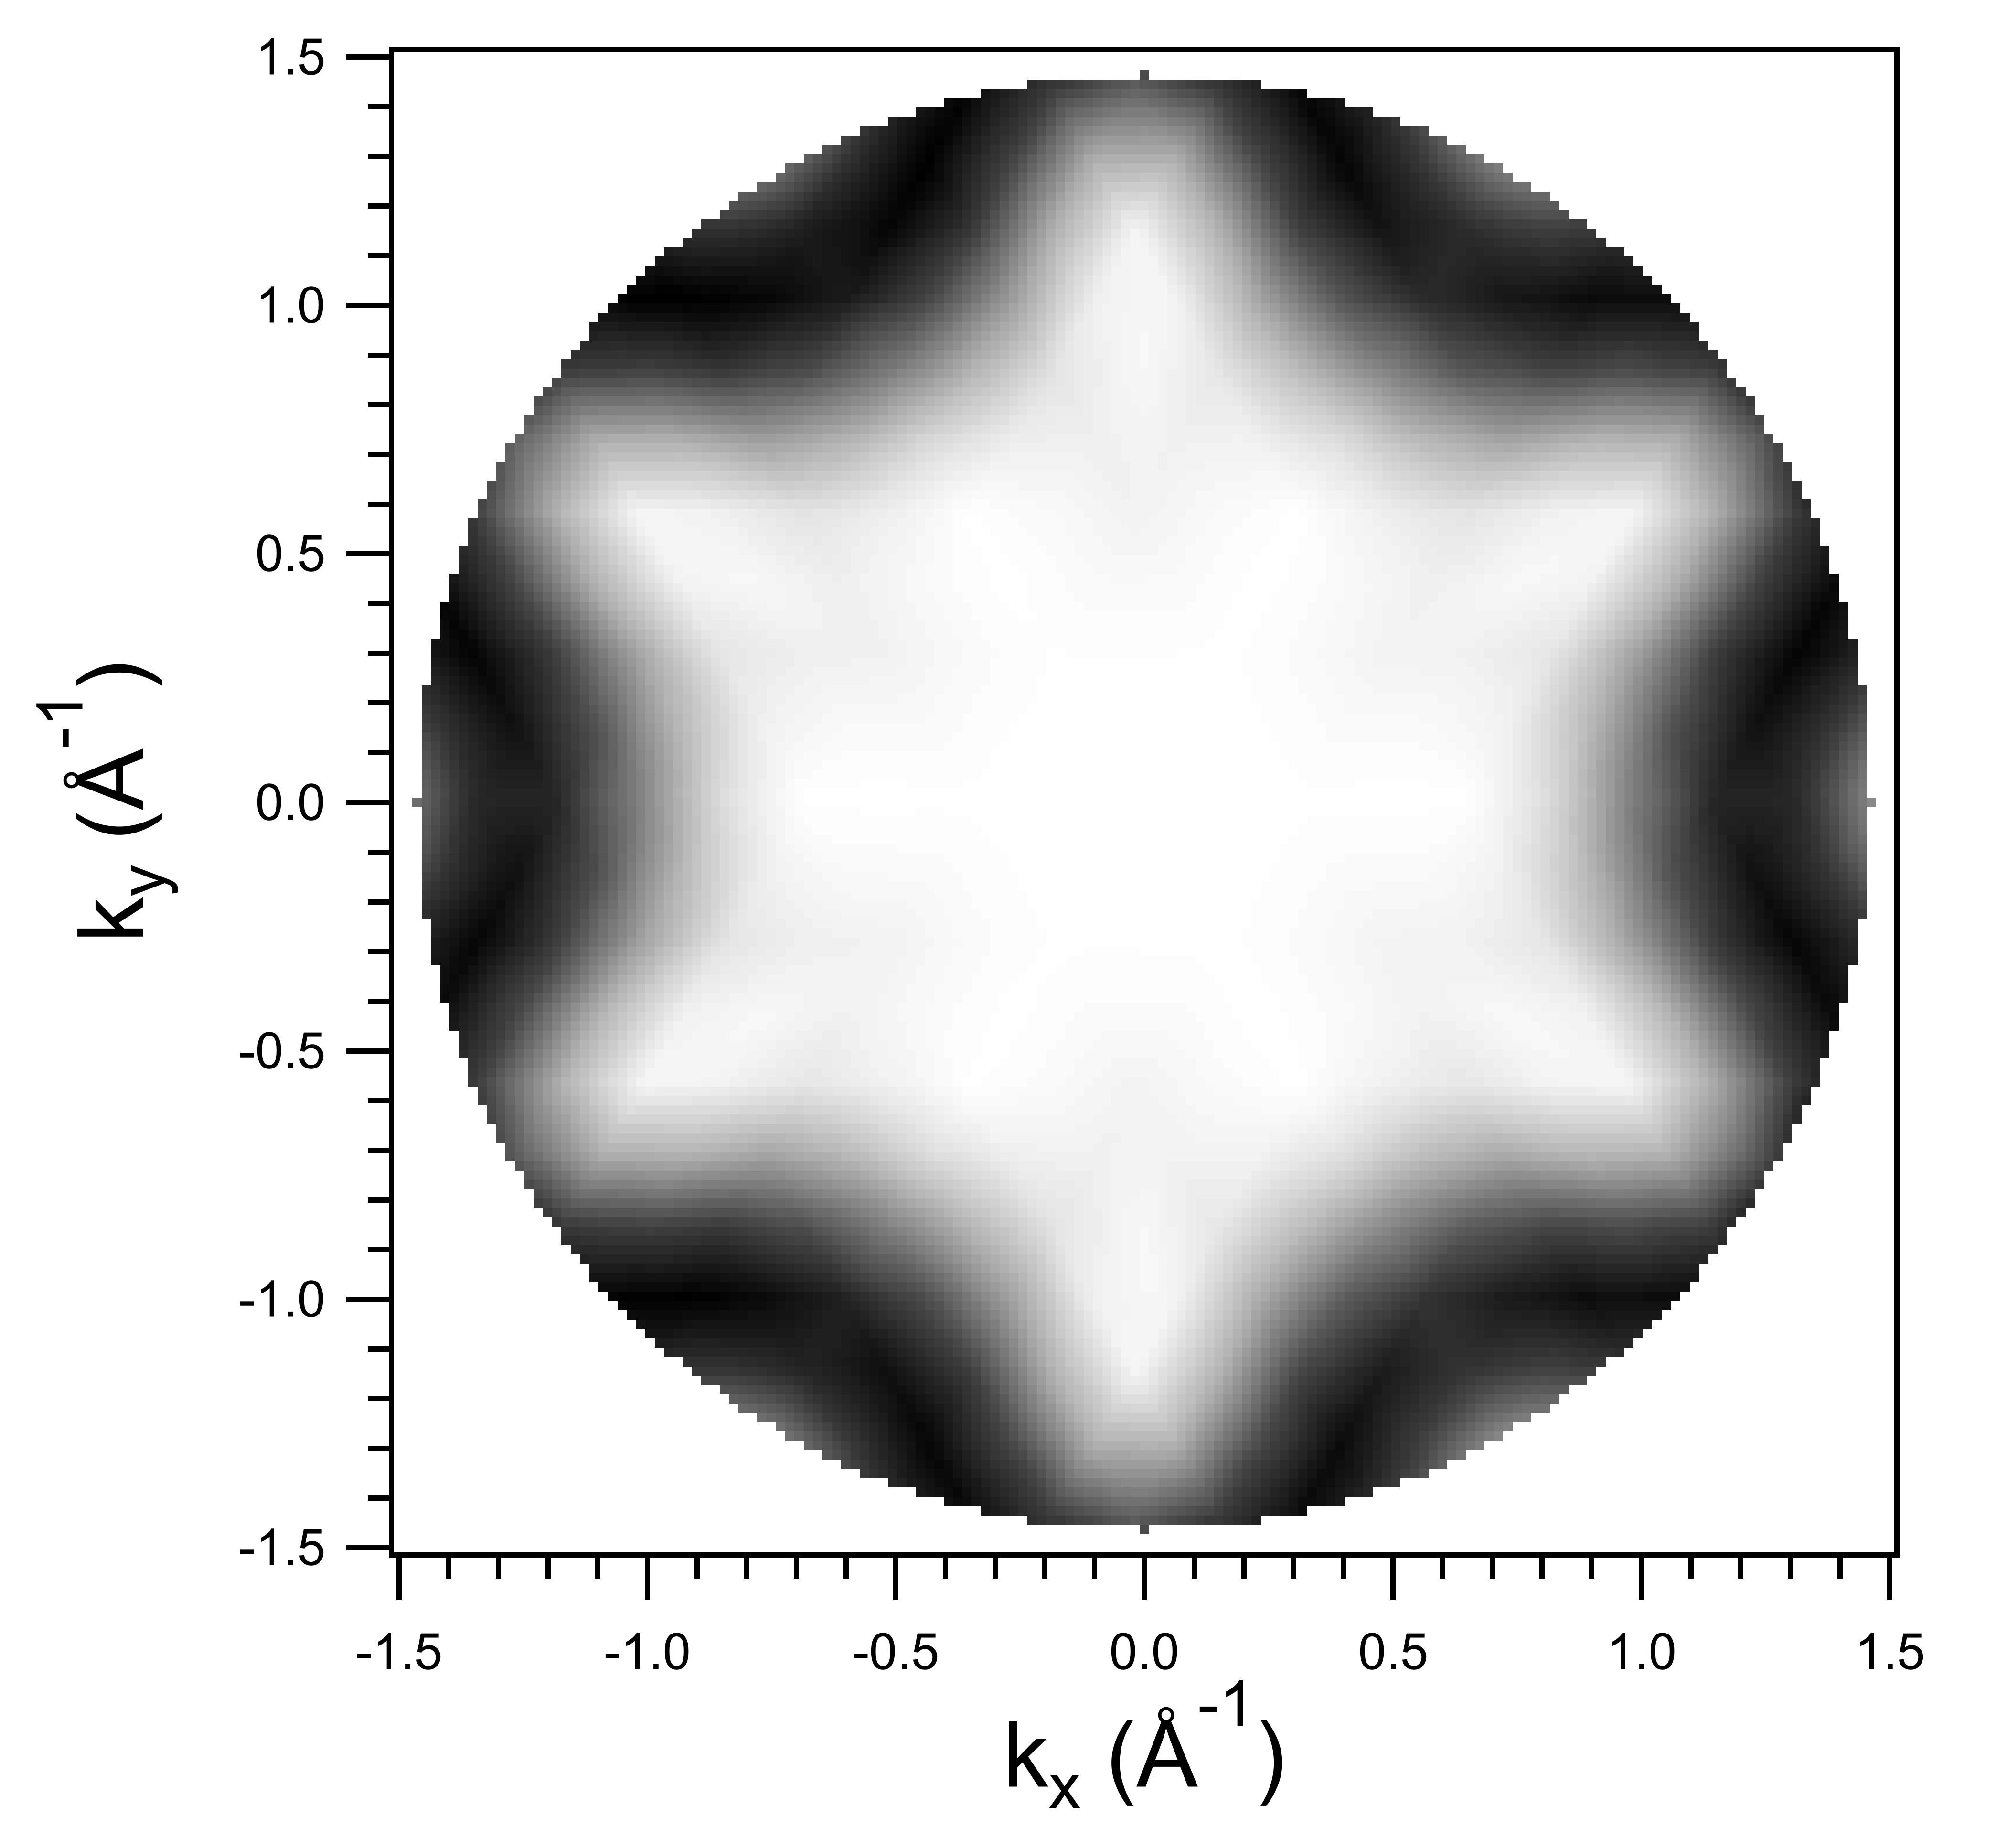
\includegraphics[height=5cm]{./content/Au+5A/HOMO1_all_CT}
                    \subcaption{Theorie Oribtale mit symmetrisierung 2mal um 120 Grad gedreht und zum Ursprungsbild addiert.}
                \end{subfigure}
                \caption{Zuordnung eines Bildes zu einem der Molekülorbitale.}
            \end{figure}
            % \begin{figure}
            %     \centering
            %     \begin{subfigure}{0.48\textwidth}
            %         \centering
            %         \includegraphics[height=5cm]{./content/Au+5A/IMAGE_2021_06_17_006_BE1_85.pdf}
            %         \subcaption{Gemmesen, symmetrisiertes Bild bei einer Bindungsenergie von \SI{1.85}{\electronvolt}.}
            %     \end{subfigure}
            %     \begin{subfigure}{0.48\textwidth}
            %         \centering
            %         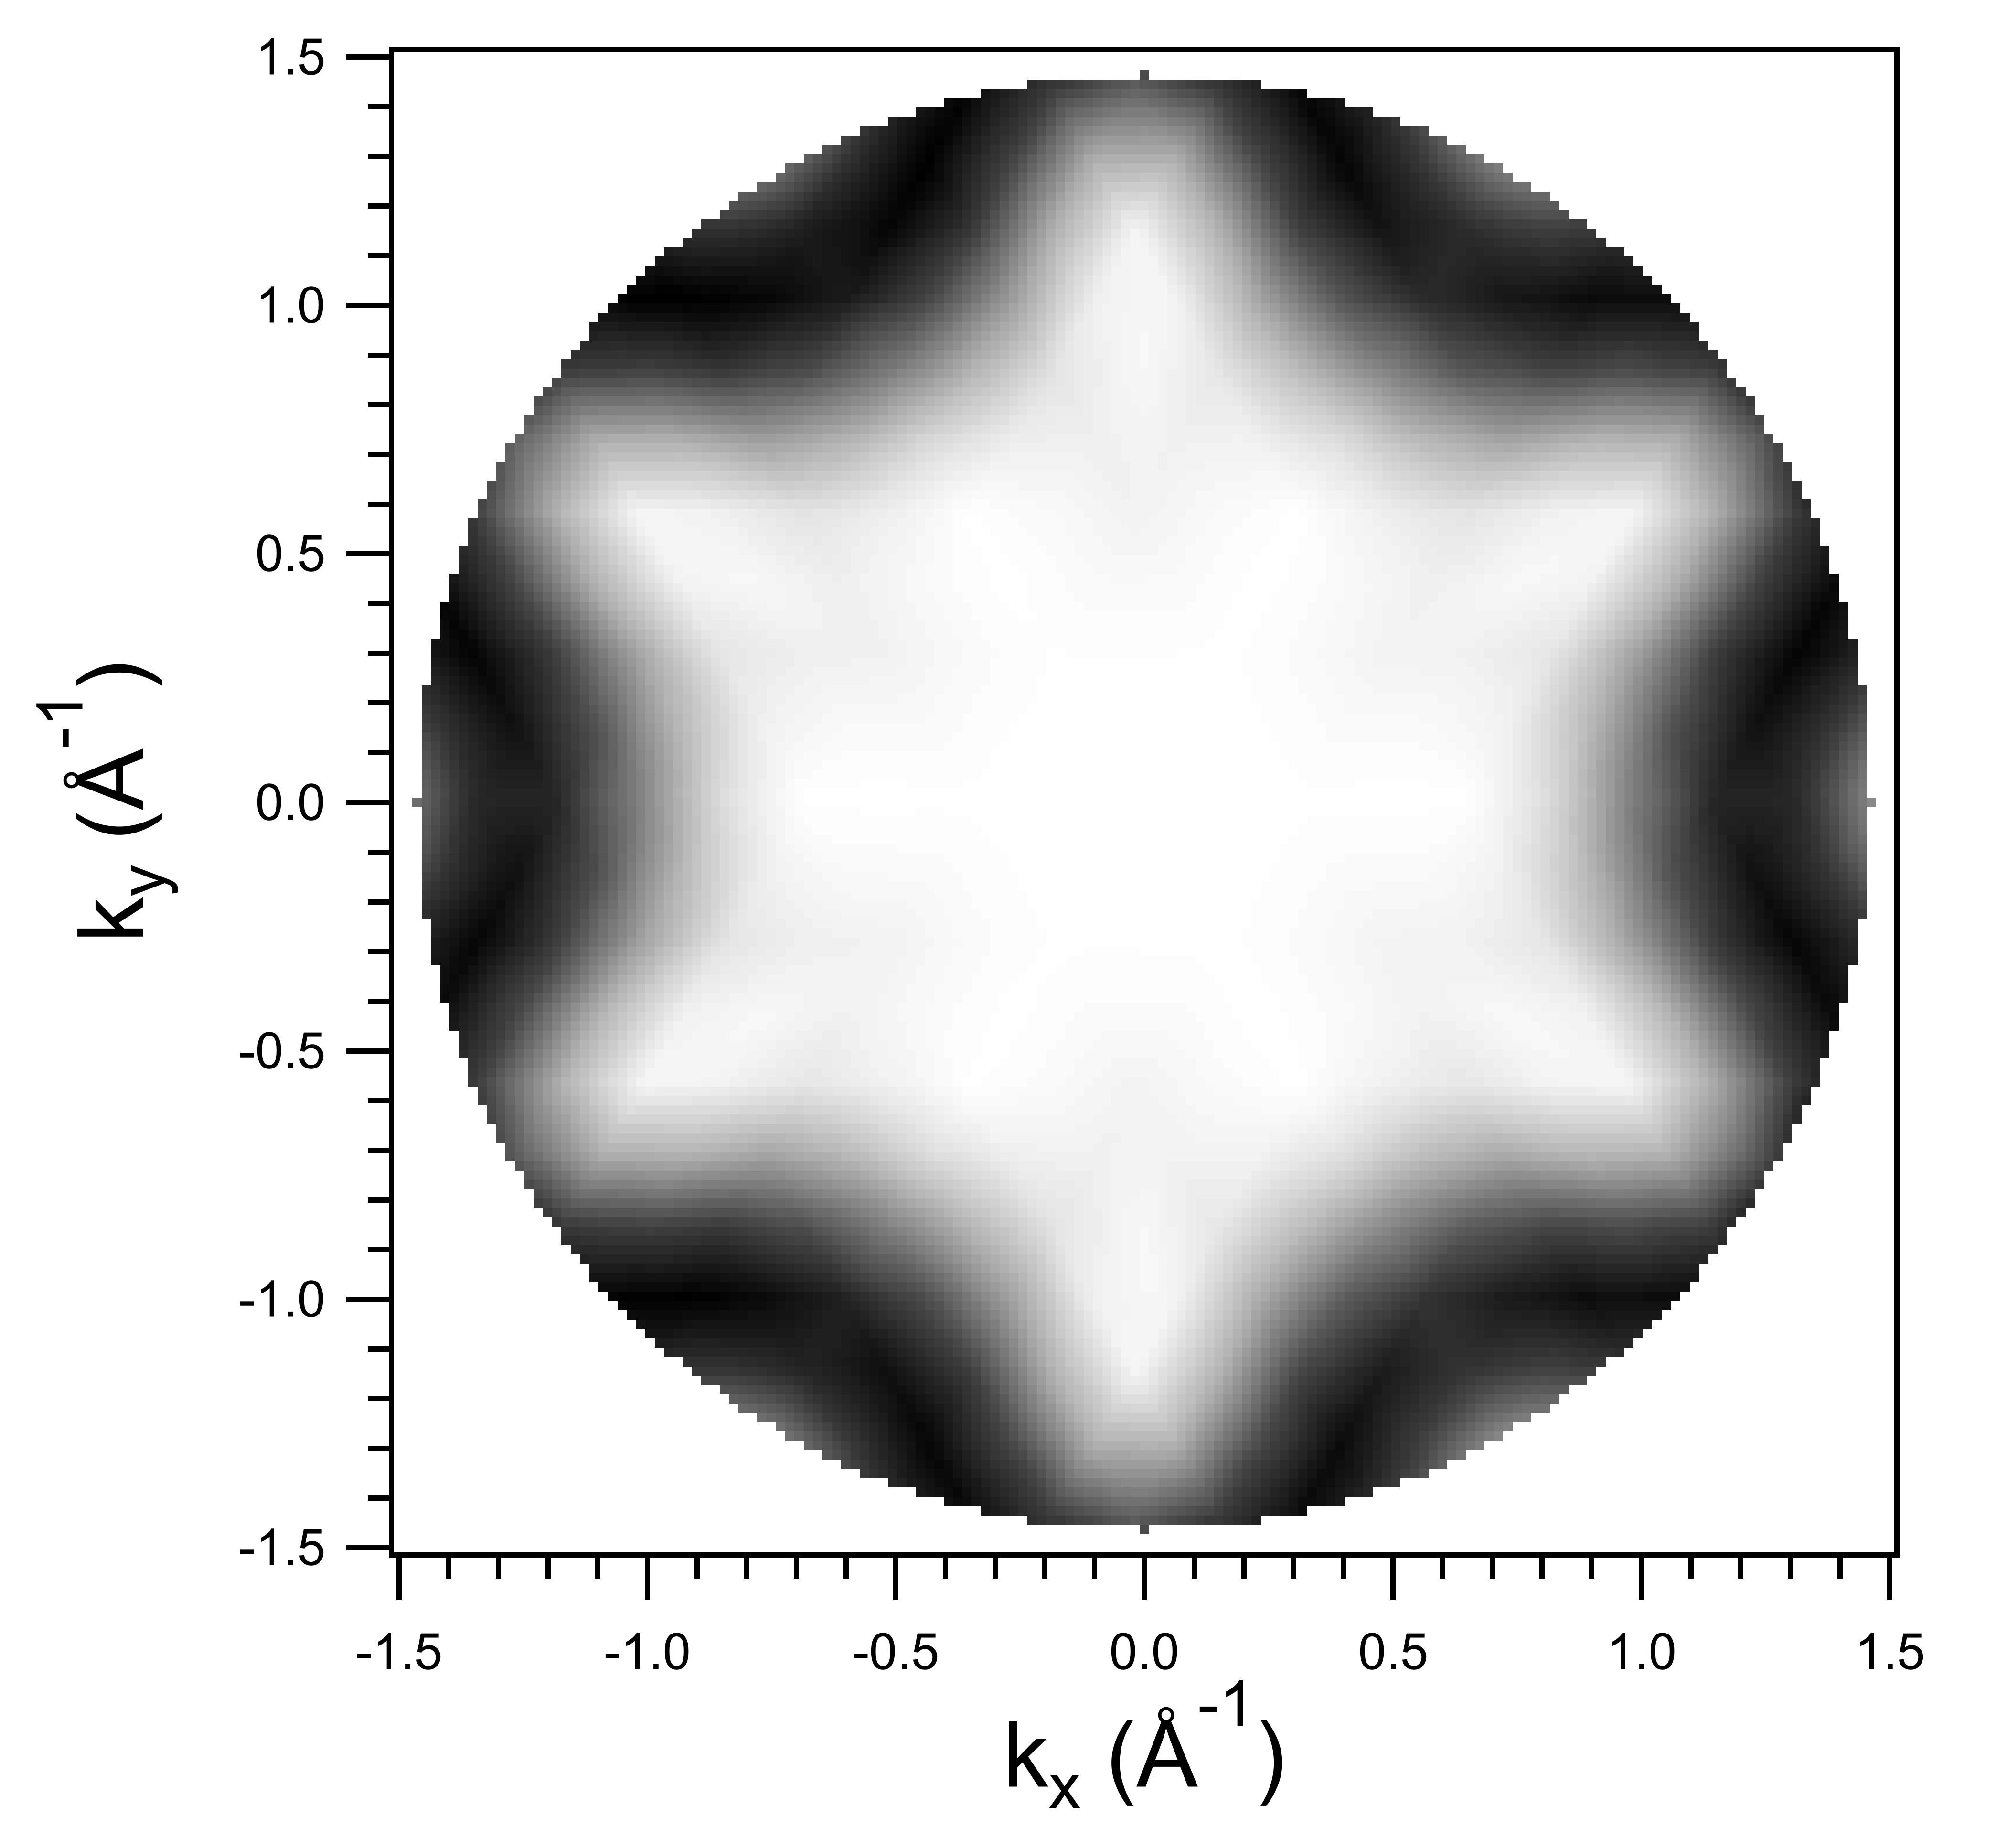
\includegraphics[height=5cm]{./content/Au+5A/HOMO1_all_CT.pdf}
            %         \subcaption{Theorie Oribtale mit symmetrisierung 2mal um 120 Grad gedreht und zum Ursprungsbild addiert.}
            %     \end{subfigure}
            %     \caption{Zuordnung eines Bildes zu einem der Molekülorbitale.}
            % \end{figure}
            % \begin{figure}
            %     \centering
            %     \begin{subfigure}{0.48\textwidth}
            %         \centering
            %         \includegraphics[height=5cm]{./content/Au+5A/IMAGE_2021_06_17_007_BE2_65.pdf}
            %         \subcaption{Gemmesen, symmetrisiertes Bild bei einer Bindungsenergie von \SI{2.65}{\electronvolt}.}
            %     \end{subfigure}
            %     \begin{subfigure}{0.48\textwidth}
            %         \centering
            %         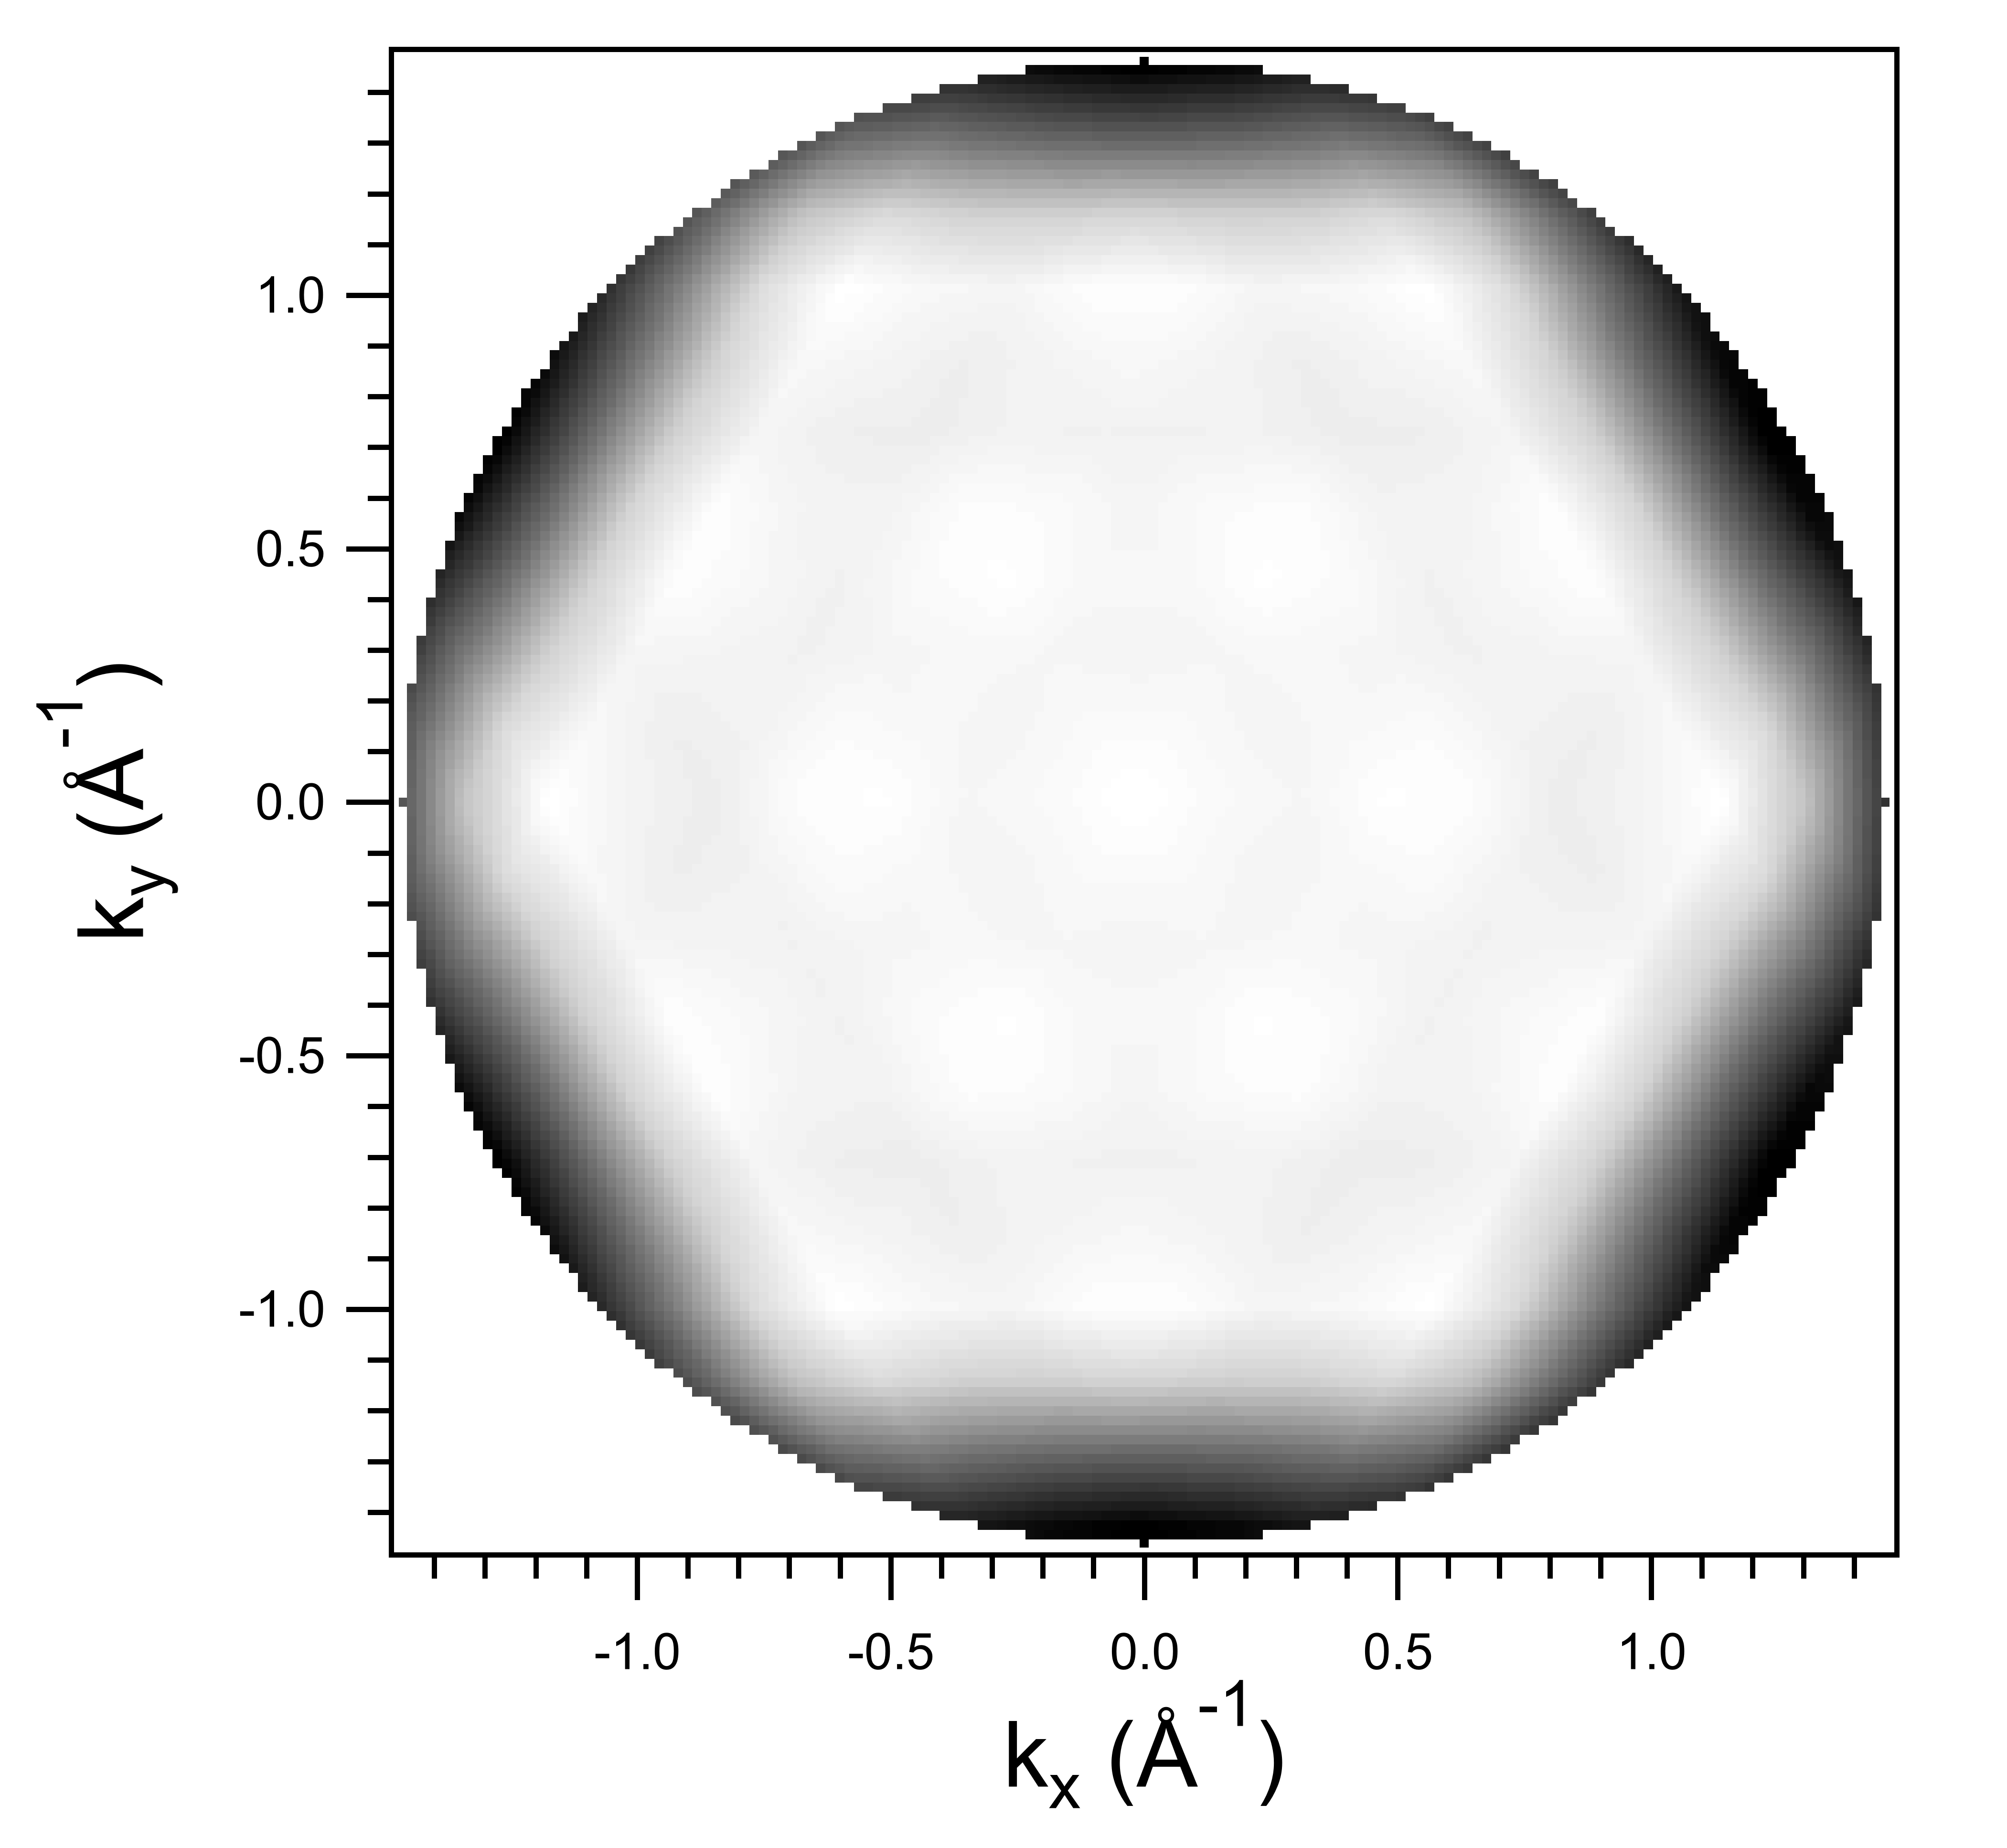
\includegraphics[height=5cm]{./content/Au+5A/HOMO2_all_CT.pdf}
            %         \subcaption{Theorie Oribtale mit symmetrisierung 2mal um 120 Grad gedreht und zum Ursprungsbild addiert.}
            %     \end{subfigure}
            %     \caption{Zuordnung eines Bildes zu einem der Molekülorbitale.}
            % \end{figure}